\documentclass[a4paper,12pt]{article}

% Packages
\usepackage[utf8]{inputenc}
\usepackage[T1]{fontenc}
\usepackage{geometry}
\usepackage{graphicx}
\usepackage[hidelinks]{hyperref}
\usepackage{amsmath}
\usepackage{amsthm}
\usepackage{amssymb}
\usepackage{bbm}
\usepackage{float}
\usepackage{booktabs}
\usepackage{siunitx}

\usepackage[backend=biber,style=numeric,citestyle=numeric]{biblatex}
\addbibresource{references.bib}

\theoremstyle{definition}
\newtheorem{theorem}{Theorem}
\newtheorem{definition}{Definition}
\newtheorem{remark}{Remark}

% Page setup
\geometry{margin=1in}

% Title
\title{Synthetic turbulent velocity field using statistics}
\author{Samy Braik}
\date{\today}

\begin{document}

\maketitle

%\begin{abstract}
% Brief summary of your report.
%\end{abstract}

\newpage
\tableofcontents
\newpage

\section{Introduction}
Turbulence is the term used to describe the unpredictable and complex behavior of a fluid's motion. It is characterized by vortex. It is opposed to a laminar flow, where the particles' movement is pre. Formally, the behavior of a fluid is quantified by the Reynolds number (Re), the higher this number is the more turbulence the fluid is. 

\bigskip

In this work, we study an ideal type of turbulence flow called Homogeneous and Isotropic Turbulence (HIT). \\
There are few properties that characterized this type of flow. It is homogeneous which means that the statistical properties (mean, variance, correlation functions) do not depend on position in space, and it is isotropic which means that these statistics are invariant under rotations or reflections of the coordinate.\\

\begin{figure}[H]
    \centering
    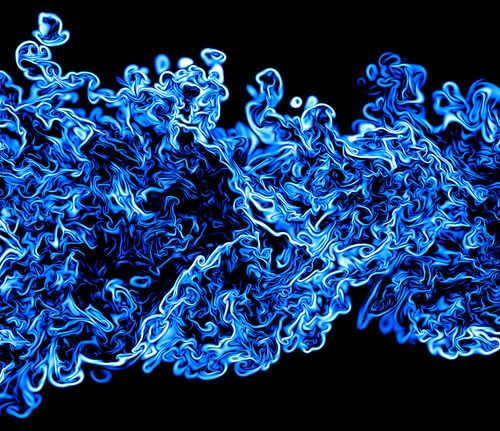
\includegraphics[width=0.7\textwidth]{illustrations/TurbulenceExample.jpg}
    \caption{Slice through the field of the scalar dissipation reveals the small-scale structure of turbulence from CNRS UMR 6614 CORIA and JSC}
\end{figure}

%First, the spatial average should be 0 for each component. Since the flow is isotropic, the turbulence properties should remain invariant to translation or axis rotations.

\bigskip

When the goal is to use statistical methods to produce turbulent velocity field two paths are worth considering. The first one is to simply use a statistical method that generate the velocity field directly. This is done in \cite{Yousif_Yu_Lim_2022},\cite{wang2025fourierflowfrequencyawareflowmatching} or \cite{parikh2025conditionalflowmatchinggenerative}. \\
Here, generative models seem the most suitable. Two major difficulties could be encountered, the huge cost and the poor generalization of the method. Indeed, in order to train such a model, there is a need for highly resolved turbulence usually produced with Direct Numerical Simulation (DNS) which are costly numerical methods. Apart from that, there is the natural cost of the method itself that can't be sidelined. The poor generalization of the method stem from the fact that usually, the models are trained on fields with a specific Reynolds number which leads to poor robustness if the turbulence parameters are changed. \\
The other path would be to start from an already existent method. For example in the case of Reynolds-averaged Navier–Stokes equations (RANS) technique (see \cite{} for details), we can use statistical methods to learn a closure model, like it is done in \cite{Bezgin2021}. This allows a better theoretical guarantee on the produced and also get rid of the robustness problem from the previous case.  

%\newpage

\section{Model}

\subsection{Random Fourier}

We set ourselves in the random Fourier model developed in \cite{Janin2021} and briefly remind it. 
Some papers that study turbulence start from a velocity field generated by DNS and use Fourier transform to study the field properties in the spectral space. The motivation behind this model, is to perform an inverse Fourier transform to generate a synthetic turbulent field with a good choice of Fourier coefficient. \\
This leads to the following expression of the velocity field 

\begin{align}
    u^s(x,t)=\int_{-\infty}^\infty\int_{-\infty}^{\infty}\left[ \hat{u}(\kappa,\omega)e^{l\psi(\kappa,\omega)}\sigma(\kappa,\omega) \right] e^{l(\kappa\cdot x + \omega t)} d\kappa d\omega
\end{align}
Discretizing the expression in N random Fourier modes and taking into account that the field is real, it could be written 
\begin{align}
    u^s(x,t)= 2 \sum_{i=1}^N \hat{u}_n \cos(\kappa^n\cdot x + \psi_n + \omega_n t)\sigma^n
\end{align}
Furthermore, we place ourselves in the following work in a froze turbulence which means that we ignore the effect of time. Therefore, the expression if simplified and we have
\begin{align}
    u^s(x,t)= 2 \sum_{n=1}^N \hat{u}_n \cos(\kappa^n\cdot x + \psi_n)\sigma^n
\end{align}
For each $n^{th}$ Fourier mode associated with the wave vector $\kappa^n$, $\hat{u}_n$ is the amplitude, $\psi_n$ the phase, $\sigma^n$ the direction and $\omega_n$ the time-frequency. \\
Like previously mentioned, a good choice of the Fourier coefficient is needed in order to produce a realistic velocity field. \cite{Janin2021} features a discussion on the choice of $\hat{u}, \kappa, \psi_n$ and $\sigma$.

\begin{figure}[H]
    \centering
    \begin{minipage}{0.49\textwidth}
        \centering
        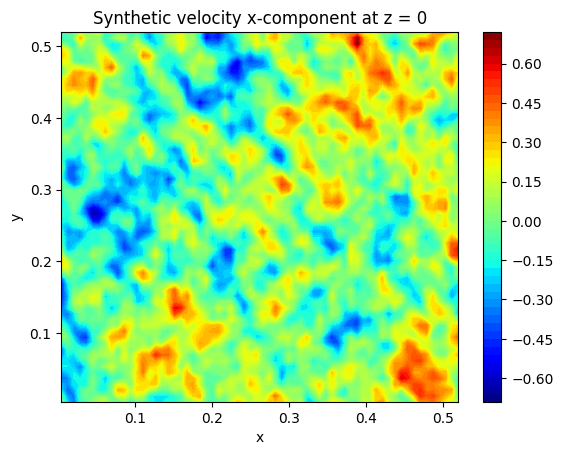
\includegraphics[width=\linewidth]{illustrations/Velocity_Example.png}
    \end{minipage}
    \hfill
    \begin{minipage}{0.49\textwidth}
        \centering
        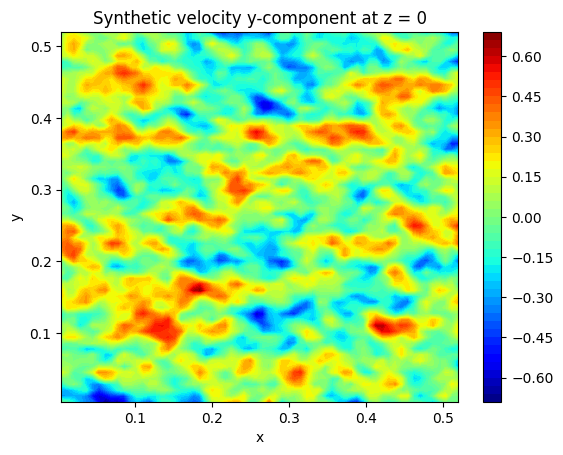
\includegraphics[width=\linewidth]{illustrations/Velocity_Example2.png}
    \end{minipage}
    \caption{Synthetic velocity obtain using the Random Fourier model}
\end{figure}

\subsection{Coefficient choice}
To ensure the statistical isotropy of the generated field, the wave vector $\kappa$ is chosen randomly on the half-sphere.
This leads to the following components choices
\begin{align}
    \kappa_1 &= \sin(\theta)\cos(\varphi) \\
    \kappa_2 &= \sin(\theta)\sin(\varphi) \\
    \kappa_2 & = \cos(\theta)
\end{align}
with the angles chosen randomly according to the following probability density functions $f_\theta(x)=\frac{sin(x)}{2}$ and $f_\varphi(x)=\frac{1}{2\pi}\mathbbm{1}_{[0,2\pi]}$. \\
Regarding the choice of $\sigma$, it is such that $\kappa\cdot\sigma=0$ is verified, which is implied by the divergence-free condition $\nabla\cdot u^s=0$. \\
Therefore, 
\begin{align}
    \sigma_1&=\cos(\varphi)\cos(\theta)\cos(\alpha)-\sin(\varphi)\sin(\alpha) \\
    \sigma_2&=\sin(\varphi)\cos(\theta)\cos(\alpha)+\cos(\theta)\sin(\alpha) \\
    \sigma_3&=-\sin(\theta)\cos(\alpha)
\end{align}
with $\alpha$ chose according to a uniform distribution on $[0,2\pi]$ i.e. $f_\alpha(x)=\frac{1}{2\pi}\mathbbm{1}_{[0,2\pi]}$. \\
The phase coefficient $\psi$ is randomly chosen according to $\mathcal{U}[0,2\pi]$ to ensure spatial homogeneity. \\
Lastly, the amplitude $\hat{u}_n=\sqrt{E(\kappa_n)\delta \kappa_n}$ where $\delta \kappa_n = \frac{\log(\kappa_N)-\log(\kappa_1)}{N}$ and $\kappa_n=e^{(\log(\kappa_1)+n\delta \kappa_n)}$. \\
The method to compute the prescribed energy spectrum $E(\kappa_n)$ is described in the next subsection.

\subsection{Energy spectrum}
%In a turbulent setup, an energy cascade is observed where a transfer of energy from large eddies to small scales (or sometimes the opposite). \\
Large eddies that carry energy distribute it through the energy cascade to smaller scales until it's dissipated by viscous effect at Kolmogorov scales. 
This energy transfer across different scales is characterized by the energy spectrum, noted $E(\kappa)$. It describes how much kinetic energy is attached to a give wave number $\kappa$. 
\begin{figure}[H]
    \centering
    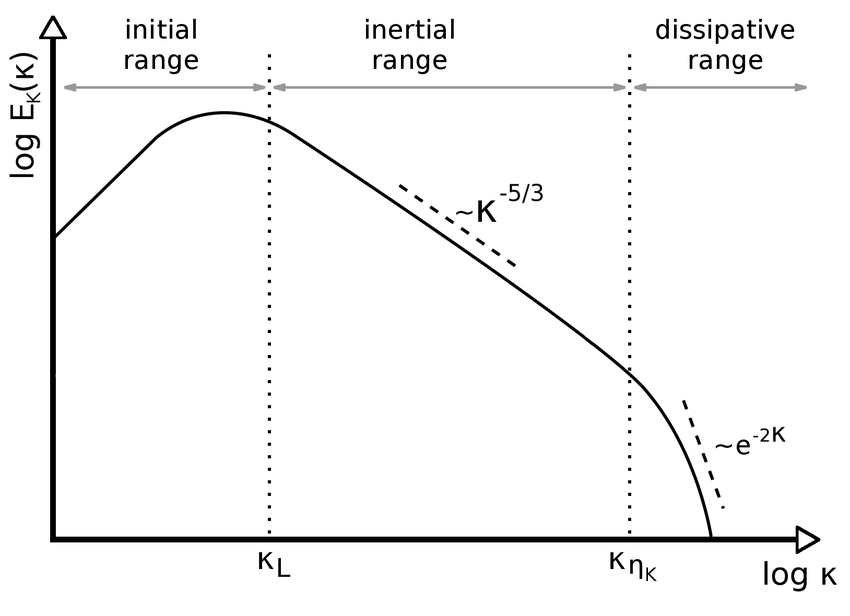
\includegraphics[width=0.7\textwidth]{illustrations/energy-spectrum-example.png}
    \caption{Energy spectrum of a turbulent flow from \cite{phdthesisRies}}
\end{figure}

In the initial range, this is where the energy is injected into the flow. Could be from an obstacle, a rotating machinery or other phenomenon. The flow is being dominated with big whirlpools. \\
The inertial range is transferred. The big whirlpools are being broke down into smaller whirlpool and so on.  

\bigskip

In the context of homogeneous isotropic turbulence, Kolmogorov gave the following formula  

\begin{align}
    E(\kappa) = C_k \kappa^{-5/3}\varepsilon^{2/3}
\end{align}
where $\varepsilon$ is the turbulent dissipation, $\kappa$ the wave number and $C_k$ the Kolmogorov constant.

Although, this formula captures the behavior in the inertial range and introduces this famous $-\frac{5}{3}$ decreases, it fails at reconstructing the spectrum in the initial and dissipative range i.e. at low and high wave numbers. To obtain a more complete recovery of the energy spectrum, \cite{Janin2021} uses, among others, the von-Kármán Pao (VKP) energy spectrum.
\bigskip

It is defined by 

\begin{align}
    E_{\text{VKP}}(\kappa)=\frac{2}{3}\alpha_e k L_e \frac{(kL_e)^4}{[(kL_e)^2+1]^{17/6}}\exp(-2(\kappa L_\eta)^2)
\end{align}

\begin{figure}[H]
    \centering
    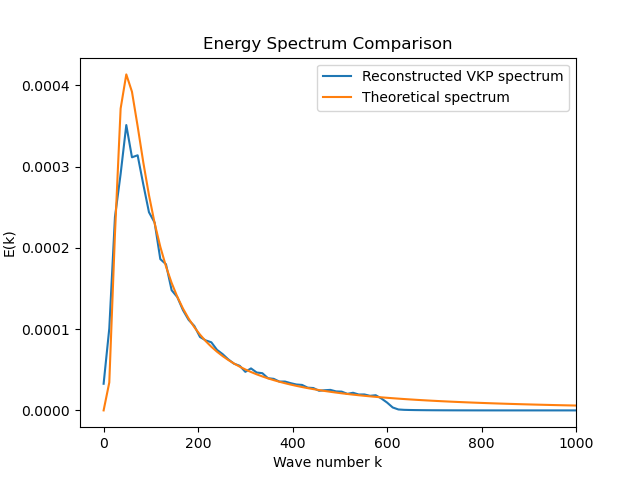
\includegraphics[width=0.7\textwidth]{illustrations/Energy_Spectrum_VKP.png}
    \caption{VKP energy spectrum vs theoretical spectrum}
\end{figure}

The real energy can be then computed 

\begin{align}
    E = \int_{0}^{\infty}E_{\text{VKP}}(\kappa) d\kappa
\end{align}

\subsection{Limitations and goals}
The assessment of the synthetic velocity field's quality could be done by looking at few metrics. First, the reconstructed energy spectrum should match as close as possible the theoretical spectrum. Then, for each component, the average should be 0 and the Root Mean Square (RMS) values should match the one used to build the turbulence in the first place. Lastly, we look at the shape of the velocity increments.   

\bigskip
Although, the model retrieve the correct energy spectrum and limited anisotropy, the velocity increments obtained are Gaussian. It is known that velocity increments appear to be non-Gaussian and more particularly heavy-tailed distribution. For instance \cite{} [Trouver un papier qui montre que pour un certain niveau de turbulence (Reynolds disons), regarder un r particulier et montre un beau plot].

\bigskip
With the random Fourier model in mind, the goal is to identify which coefficient could lead to more realistic velocity increments without disrupting the other good properties that are already satisfied. 


\section{Method}
To tackle the problem, no obvious path stood out. 
The one chosen is simply to define a model and a loss and optimize the model's parameters. \\
Since the goal was to retrieve heavy-tailed velocity increments, the logical criteria to look out was the kurtosis of those increments. 

[Mieux décrire le model (nn.Parameter)]

\begin{definition}[Kurtosis]
    Let $X$ be a real random variable, $\mu$ its mean and $\sigma$ its standard deviation. Its kurtosis is defined by 
    \begin{align}
    \beta_2=\mathbb{E}\left((\frac{X-\mu}{\sigma}) \right)^2    
    \end{align}
     
\end{definition}

\begin{remark}
    For a Gaussian distribution, which is the distribution of the velocity increments in the first place, the kurtosis is equal to 3.
\end{remark}

\begin{remark}
    In practice, we look at the flatness which is simply the $\beta_2-3$.
\end{remark}

\subsection{Preliminary work}
In order to check the robustness of the model in the first place, we conducted a simple experiment. We set the target flatness as 3, meaning we look for Gaussian velocity increments. Starting from Gaussian velocity increments and heavy-tailed velocity increments, the goal is to see if we can retrieve (or in the first place keep) Gaussian velocity increments.  


\subsection{Phase coefficient}
The first idea was to work on the phase parameter $\psi$. 


\subsection{Phase, wave vector and direction}

\subsection{Angles}


\section{Results and Discussion}
The work was highly exploratory and featured trials and errors along the way.

\section{Conclusion}
% Conclusion and future work.

\appendix

\section{Turbulence parameters}
To generate the turbulence few physical and spectral parameters have to be given as input for the model. Throughout the report the parameters that have been used are listed in the following table. 

\begin{center}
\begin{tabular}{lll}
\toprule
\textbf{Parameter} & \textbf{Value} & \textbf{Unit}\\
\midrule
Length of the periodic box   & $\tfrac{\pi}{6}$ & \si{\meter}\\
Number of modes              & 250 or 500 & --\\
RMS speed                    & 0.222 & \si{\meter\per\second}\\
Integral length scale        & 0.024 & \si{\meter} \\
Kinetic energy               & $1.5 \times (0.222 \times 2)$ & \si{\meter\squared\per\second\squared} \\
Viscosity                    & $1.8 \times 10^{-5}$ & \si{\meter\squared\per\second} \\
Minimum wave number          & $\tfrac{2\pi}{1.0}$ & \si{\per\meter}\\
Maximum wave number          & $\tfrac{2\pi}{0.01}$ & \si{\per\meter}\\
\bottomrule
\end{tabular}
\end{center}

\section{Coefficient marginal distributions}


\newpage
\printbibliography

\end{document}